\chapter{Y00-量子暗号システム}
Y00-量子暗号のシステムについて説明する。送信者と受信者はseedkeyを共有している。まずLFSRによって疑似乱数を発生させる。
このとき、seedkeyが同じであるので発生する乱数も同じとなる。乱数は基底番号を表し、送信者と受信者は同じ基底番号を使うことができる。送信器では送信バイナリデータと基底番号の値に対応する量子状態を送信する。受信器では受け取った量子状態と基底番号を使ってバイナリデータを出力する。次に受信機における処理について説明する。

\begin{figure}[htbp]
        \centering   
        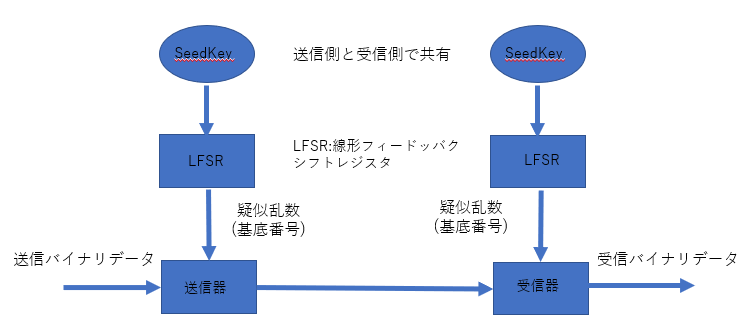
\includegraphics[width=1.0\textwidth]{img/zemi3.png}
        \caption[sample image (png)]{量子暗号システム.}
        \label{fig:4_1}
    \end{figure}



受信器ではまずホモダイン測定を行う。ホモダイン測定はコヒーレント状態の複素振幅$\alpha=x+iy$成分を測定する。\figref{Fig:4_2}は0と1に対応するコヒーレント状態をホモダイン測定した場合の出力の確率分布である。それぞれの分布は分散1/4の正規分布になっている。受信器では、測定値に基づき、しきい値を使って受信したデータが0か1か判断する。

\begin{figure}[htbp]
        \centering   
        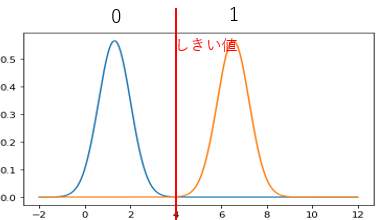
\includegraphics[width=0.7\textwidth]{img/zemi4}
        \caption[sample image (png)]{ホモダイン測定.}
        \label{Fig:4_2}
    \end{figure}
    
\figref{Fig:4_3}は受信機のしきい値処理を説明したものである。2つのコヒーレント状態の値のちょうど真ん中をしきい値とする。基底番号が3の場合それに対応するコヒーレント状態は緑色に示したコヒーレント状態になるが、そのときのしきい値は$\frac{S_{max}}{2B-1}(\frac{B}{2}+k)$となる。また、基底番号が奇数の場合、測定値がしきい値より大きければ1、小さければ0と判定する.基底番号が偶数の場合、測定値がしきい値より大きければ0、小さければ1と判定する。

\begin{figure}[htbp]
        \centering   
        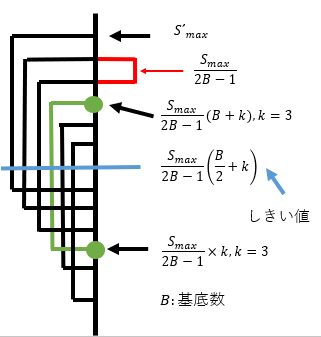
\includegraphics[width=0.5\textwidth]{img/zemi5.png}
        \caption[sample image (png)]{受信機のしきい値処理.}
        \label{Fig:4_3}
    \end{figure}


